%----------------------------------------------------------------
%
%  File    :  vpn_evaluation.tex
%
%  Author  :  Keith Andrews, IICM, TU Graz, Austria
% 
%  Created :  22 Feb 96
% 
%  Changed :  19 Feb 2004
% 
%----------------------------------------------------------------

\chapter{Evaluation} \label{chap:Evaluation}

This chapter presents the results of our model learning and model-based fuzzing. Firstly, our environment setup is discussed in Section~\ref{sec:env}. Following that, the learning results are presented in Section \ref{sec:learnresults}, beginning with the models learned using various input alphabets. The presentation of learned models is followed by a comparison of the two used learning algorithms, $L^*$ and $KV$, as well as the discussion of a library error found during learning. Finally, the fuzzing results are presented and discussed in Section \ref{subsec:fuzzresults}, comparing the two methods of run generation introduced in Chapter~\ref{chap:Fuzzing}.

\section{Environment Setup} \label{sec:env}
% describe VMs, IPsec server software, configuration etc
All model learning and testing took place in a virtual environment using two VirtualBox 6.1 \acp{vm} running standard Ubuntu 22.04 LTS distributions. Both \acp{vm} were allotted \SI{4}{\giga\byte} of memory and one CPU core. All inter-\ac{vm} communication took place in an isolated virtual network to eliminate possible external influences. During learning and fuzzing, all power saving options and similar potential causes of disruptions were disabled. Additionally, the \ac{ipsec} server was restarted before each learning attempt to ensure identical starting conditions. One \ac{vm} was designated as the initiator and one as the responder to create a typical client-server setup. We chose the open source \ac{ipsec} implementation Strongswan\footnote{https://www.strongswan.org/} as our \ac{sul}. The Strongswan server was installed on the responder \ac{vm} and set to listen for incoming connections from the initiator \ac{vm}. We used the Strongswan version US.9.5/K5.15.0-25-generic, installed using the default Ubuntu package manager, apt. The Strongswan server was configured to use \acp{psk} for authentication and default recommended security settings. Additionally, it was configured to allow unencrypted notification messages, which we used to reset the connection during the learning process. The used Strongswan configuration files can be found in Appendix TODO \todo{appendix}. The Python library \textsc{AALpy}\footnote{https://github.com/DES-Lab/AALpy} version 1.2.9 was used in conjunction with the packet manipulation library Scapy\footnote{https://scapy.net/}, version 2.4.5, in order to learn a model of the \ac{sut}. Significant effort was put into expanding the \ac{isakmp} Scapy module to support all packets required for \ac{ipsec} as the module lacked many features out-of-the-box. The provided Python script, \todo{this}\emph{IPSEC\_IKEv1\_SUL}\footnote{TODO: github or supplementary material link} demonstrates how \textsc{AALpy} can be used in conjunction with our custom mapper to communicate with and learn the model of an \ac{ipsec} server. Figure~\ref{fig:AALSetup} shows a typical learning attempt using two connected \acp{vm}. The right \ac{vm} shows the output of an underway learning attempt, while the left one shows the corresponding Strongswan server logs.

\section{Learning Results} \label{sec:learnresults}
% section where we show and analyze reference and no filter models including model and statistics
\todo[inline]{rewrite / expand on this portion, detail exact configurations / should I detail it again if I already did so in methods?}
Over the course of our work, we learned a variety of different models due to different retransmission-handling settings and choice of inputs alphabets. The following sections showcase the four most relevant ones, all learned from a Linux Strongswan U5.9.5 server, using both the $KV$ and $L^*$ learning algorithms. Error codes have been simplified for better readability. As our \ac{sul} had some issues with non-determinism while retransmissions were enabled, one major differentiating factor in our models is whether retransmission-filtering was enabled for the learning process. This had a significant impact on the resulting learned model, with the version without filtering boasting more than twice the number of states than the one with. Additionally, even when using the methods to combat non-determinism described in Chapter \ref{chap:Learning}, Section \ref{subsec:nondet} the resulting models still occasionally differed when not filtering out retransmissions. Therefore, the non-filtered models were not used for fuzzing, as a completely deterministic model was desired to serve as our baseline when fuzzing the \ac{sut}.

\subsection{Learning Metrics} \label{subsec:metrics}
The comparison of learned models and model learning algorithm performance in subsections \ref{subsec:models} and \ref{subsec:comp_kv_lstar} is based largely on the the following metrics, saved during the model learning process.

\subsubsection*{Steps}
Steps refers to the number of algorithm steps required by the learning algorithm or the equivalence checking.

\subsubsection*{Queries}
Queries refers to the amount of queries sent during state exploration (membership queries) or during conformance checking (equivalence queries). \textsc{AALpy} supports speeding up model learning by using caching to reduce the number of required membership queries. 

\subsubsection*{Runtime}
Runtime refers to the time it took to learn the model. It is further split into state exploration and conformance checking runtimes. Runtime directly correlates to the number of steps and queries. When given in seconds, the runtime is rounded to the nearest second.


\subsection{Learned Models} \label{subsec:models}
Figures \ref{fig:ret_case1} and \ref{fig:ret_case2} show the two most commonly learned models when not filtering retransmissions. Roughly 80\% of all models learned without retransmission filtering enabled resulted in one of these two models, which we will refer to as the common models. The other 20\% of models were a non-uniform assortment of outliers. Figure \ref{fig:reference} shows the clean base model learned from the \ac{sul} with retransmission filtering enabled. The reference model used for fuzzing is shown in Figure \ref{fig:withfilterwitherrors}, also learned with retransmission-filtering enabled, as well as an expanded input alphabet. Dot files of all models are provided in Appendix \todo[inline]{APPENDIX/additional resources}.

\subsubsection*{First Common Model}

The first common model, presented in Figure \ref{fig:ret_case1}, took approximately 52 minutes (3092 seconds) to learn with the $KV$ algorithm, spread over seven learning rounds. The model consists of 10 states. Of the 52 minutes total, roughly half were used for state exploration/membership queries and the other half for conformance checking, with conformance checking taking slightly longer (1501 vs 1591 seconds). 171 membership queries were performed by the learning algorithm in 2047 steps, whereas 100 equivalence queries were performed for conformance checking in 1826 steps.

In contrast, when learned with the $L^*$ algorithm, model learning took almost 85 minutes (5094 seconds) over five learning rounds. Here, the split between state exploration and conformance checking was more distinct, with state exploration taking up approximately 68\% of the total runtime and conformance checking only requiring the remaining 32\% (3489 vs 1605 seconds). Notably, the time needed for conformance checking remained largely the same between the two algorithms, however the difference in state exploration / membership queries is quite large. This behavior is discussed in more detail in Subsection \ref{subsec:comp_kv_lstar}, which includes a statistical comparison of the two algorithms.

Moving on to an examination of the first common model itself, we can clearly see a separation between the two phases. Phase one completes in state \emph{s3}, and phase two begins right thereafter. While phase one looks very clean and is in fact identical to the model learned with retransmission-filtering enabled, phase two has many strange transitions caused by retransmissions. For example, all three transitions from state \emph{s5} to \emph{s7} via \emph{sa\_main}, \emph{sa\_main} and \emph{key\_ex\_main}, highlighted in yellow, return a valid \emph{IPSEC SA} response. This should be impossible, as phase one messages are ignored while in phase two. However, due to specific timings of retransmissions, our communication interface can occasionally happen to be listening for a server response of a regular phase two communication, when the \ac{sul} sends a retransmission for previous \emph{sa\_quick} message. This causes our framework to treat the received retransmission as the response for the phase two message, when in fact, it is not. We can see multiple incoming and outgoing transitions of state \emph{s4}, highlighted in red, that further exhibit this same same behavior.
Another noticeable property of the learned automata, is that past state \emph{s2}, no paths lead back to the initial state. This is due to the fact that we did not include the delete command in the alphabet for this learned model. Adding delete adds transitions from every state back to the initial one, but also dramatically increases the runtime and non-deterministic behavior of the \ac{sul}, as even more retransmissions are triggered. While not part of our input alphabet, it could be included in future work.

\begin{figure}[ht]
	\vspace*{\fill}
	\noindent
	\hspace*{-2.1\oddsidemargin}%
	\makebox[0pt][l]{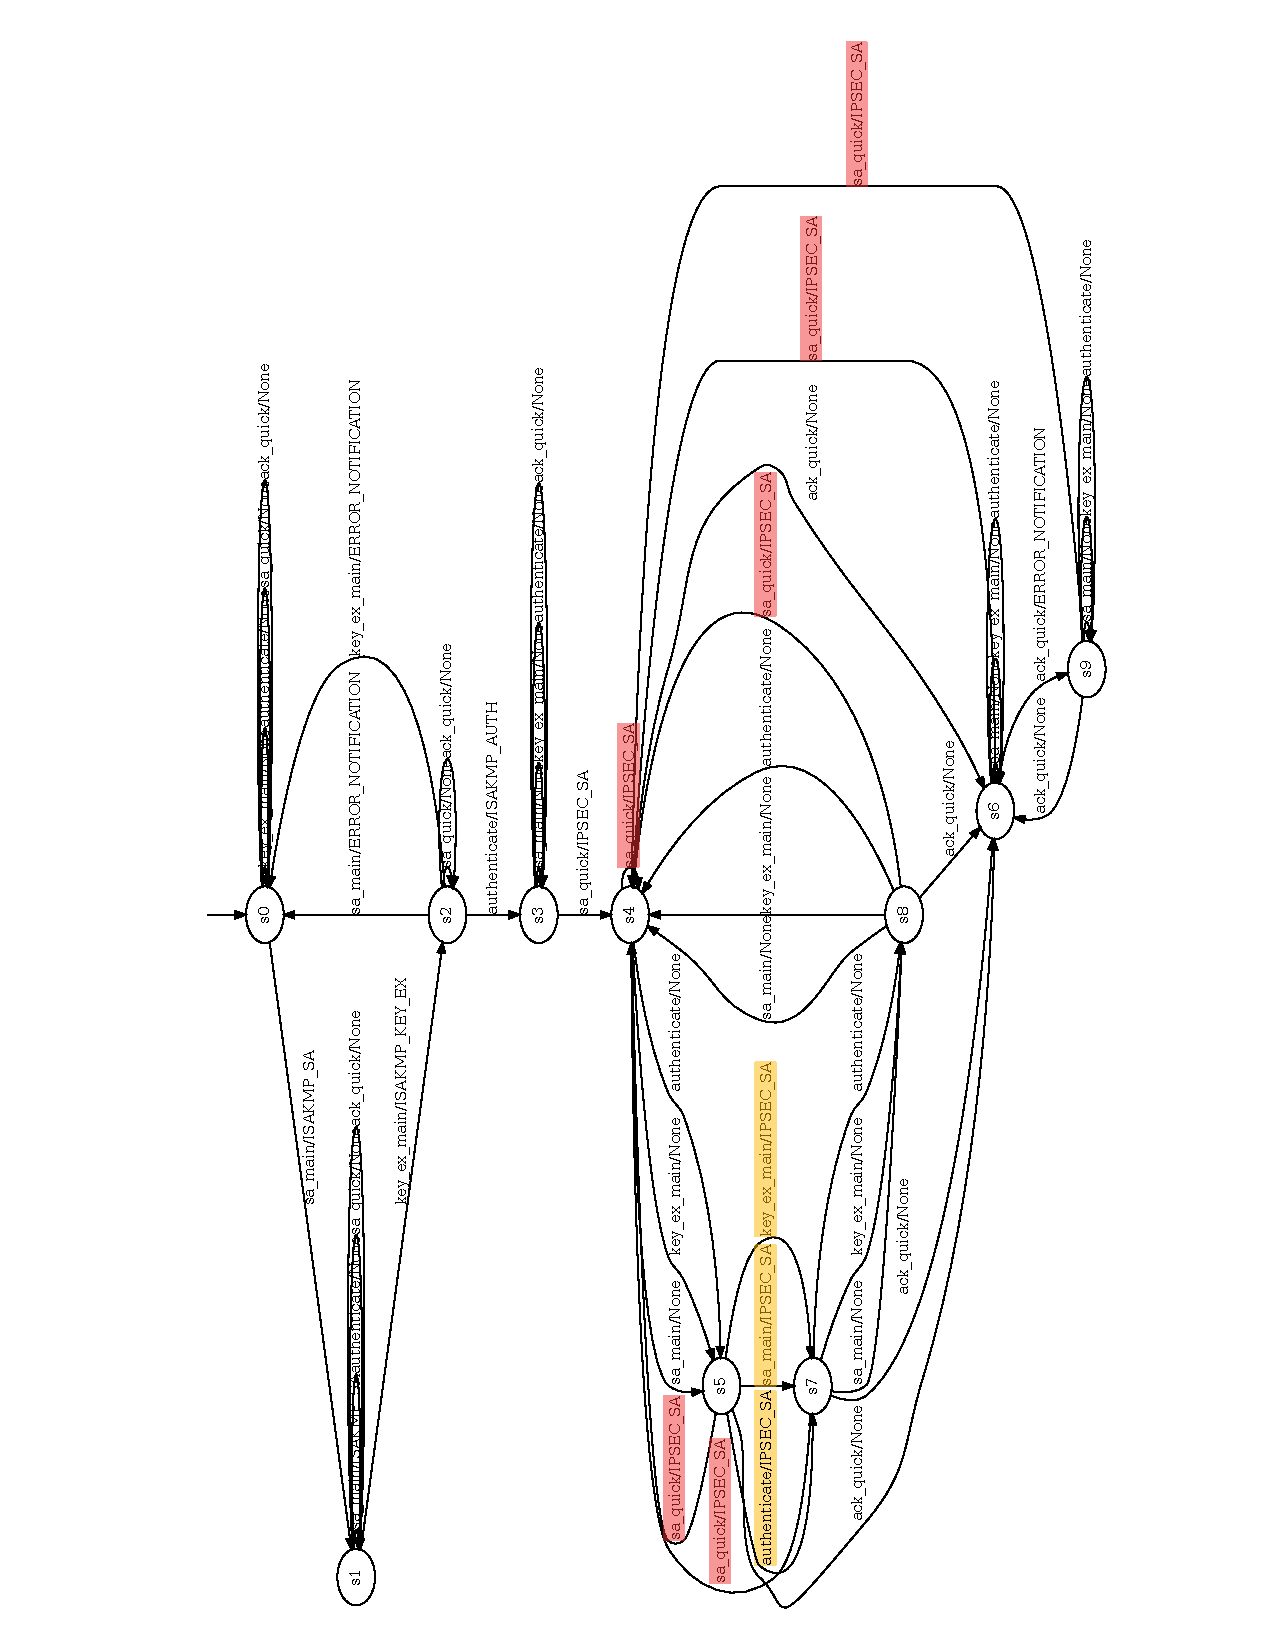
\includegraphics[width=\linewidth, angle=270]{images/models/retransmissions/retrans_case1_lstar}}
	\caption{First commonly learned model with retransmissions.}
	\label{fig:ret_case1}
	\vspace*{\fill}
\end{figure}

\newpage

\subsubsection*{Second Common Model}

The second common model, seen in Figure \ref{fig:ret_case2}, took approximately 75 minutes (4507 seconds) to learn using the $KV$ algorithm. The model took nine rounds to learn, and consists of 12 states. Of those 75 minutes, roughly 53\$ were used for state exploration / membership queries and the other 47\% (2382 vs 2126 seconds). 215 membership queries were performed by the learning algorithm in 2219 steps, whereas 120 equivalence queries were performed for conformance checking in 1964 steps. 

In contrast, when learned with the $L^*$ algorithm, model learning took significantly longer, running for 125 minutes (7520 seconds) over five learning rounds. Here, the split between state exploration and conformance checking was again very distinct, with state exploration taking up approximately 71\% of the total runtime and conformance checking only requiring the remaining 29\% (5393 vs 2126 seconds). Again, the time needed for conformance checking remained largely the same between the two algorithms, however the difference in state exploration / membership queries is even larger.

Examining the model, we can again see a clear separation between the two phases. Phase one for this model is identical to the previous one, as no retransmission occur there. Same as in Figure \ref{fig:ret_case1}, no paths past state \emph{s2} lead back to the initial state. Phase two shows retransmission-induced strange behavior in the transitions \emph{s5} to \emph{s7}, as well as \emph{s11} to \emph{s9}. The strange behavior is again linked to retransmissions, causing phase one inputs, such as \emph{sa\_main}, to result in the valid phase two outputs, such as \emph{IPSEC SA}. The states \emph{s7} and \emph{s11} are separated by two states that do not exhibit any strange behavior, apart from having identical in and outputs. The main difference to the first common model is, that strange behavior occurs in two pairs of states, highlighted in yellow, and that these pairs are separated by two states that do not appear to receive any retransmissions, highlighted in red. This is likely caused by the \ac{sut} sending repeated retransmissions, in the same frequency, allowing for two states in between. 

\begin{figure}[ht]
	\vspace*{\fill}
	\noindent
	\hspace*{-2.1\oddsidemargin}%
	\makebox[0pt][l]{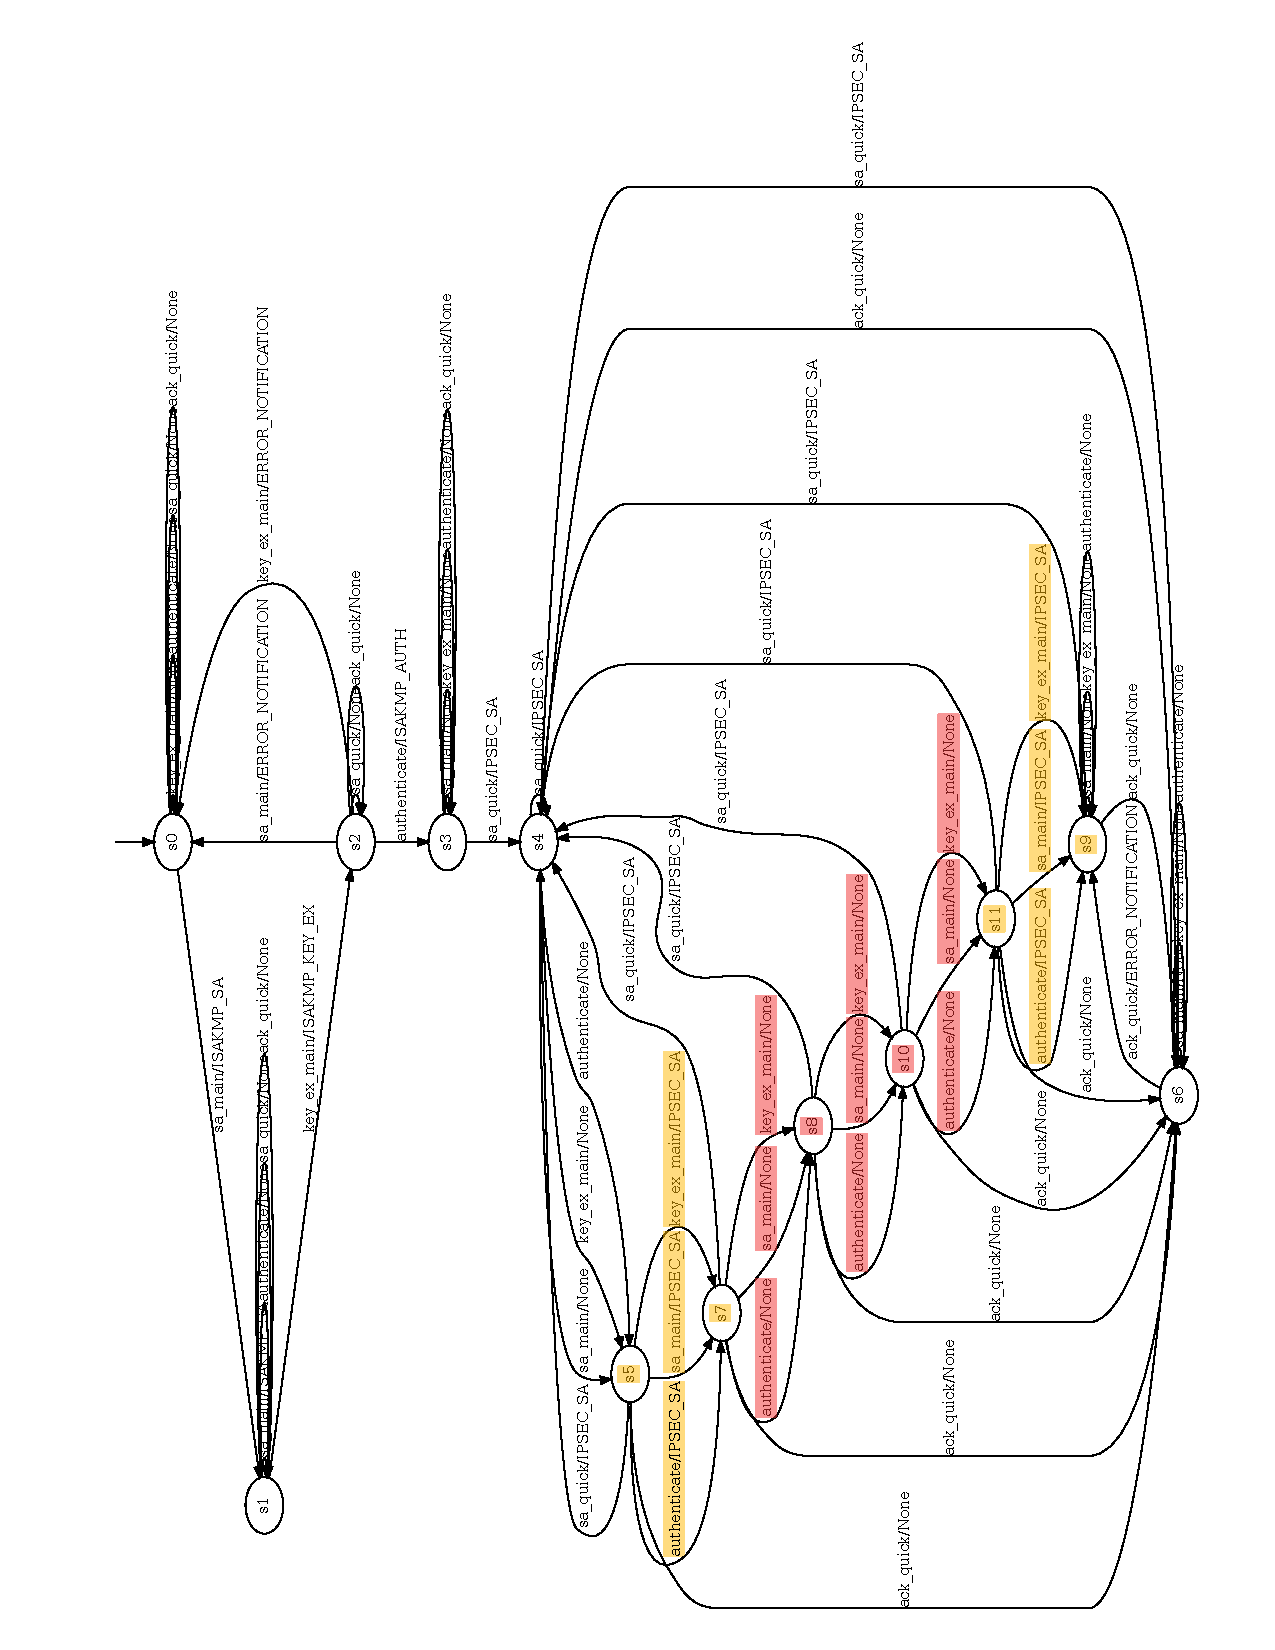
\includegraphics[width=\linewidth, angle=270]{images/models/retransmissions/retrans_case2_lstar}}
	\caption{Second commonly learned model with retransmissions.}
	\label{fig:ret_case2}
	\vspace*{\fill}
\end{figure}
\newpage

\subsubsection*{Clean Base Model}

In comparison, when learning the same server using retransmission-filtering, all non-deterministic behavior vanishes and we get the model shown in Figure \ref{fig:reference} every learning attempt. The model has only 6 states and therefore was learned much more quickly than the previous ones, with learning requiring only approximately 21 minutes (1266 seconds) using the $KV$ algorithm. Learning happened over four rounds, where the time was distributed between state exploration and conformance checking in a 60-40 split (519 vs 747 seconds). In comparison, when learned with the $L^*$ algorithm, learning took roughly 36 minutes (2157 seconds), spread over two learning rounds. Of that time, state exploration required roughly 55\% compared to the 45\% needed for conformance checking (1188 vs 969 seconds). Compared to $KV$, state exploration / membership queries took more than twice the amount of time to complete.

states \emph{s6} to \emph{s11}. In these states, we can see that phase one messages, which are usually ignored in phase two, result in \emph{IPSEC SA} responses.

Looking at the resulting model more closely, we can see that the first four states are again identical to the previous model. This is due to the fact that the retransmissions only triggered for phase two messages and since they are our only source of non-determinism, we see no differences here. However, the phase two states look wildly different, showing a streamlined behavior that fits our reference \ac{ike} exchange (see Figure \ref{fig:IKEv1}) almost perfectly. The only small difference lies in the additional state \emph{s5} which loops back to state \emph{s4} with an \emph{IPSEC SA} or \emph{ACK} message. This behavior demonstrates how one can create multiple \ac{ipsec} SAs on a single \ac{ike} \ac{sa} channel. And once a new \ac{ipsec} \ac{sa} has been established, we can again send another \emph{ACK} message. In other words, the extra state is there to show that we cannot acknowledge a single \ac{ipsec} \ac{sa} twice, but need to first create a new one.

\begin{figure}[h]
	\centering
	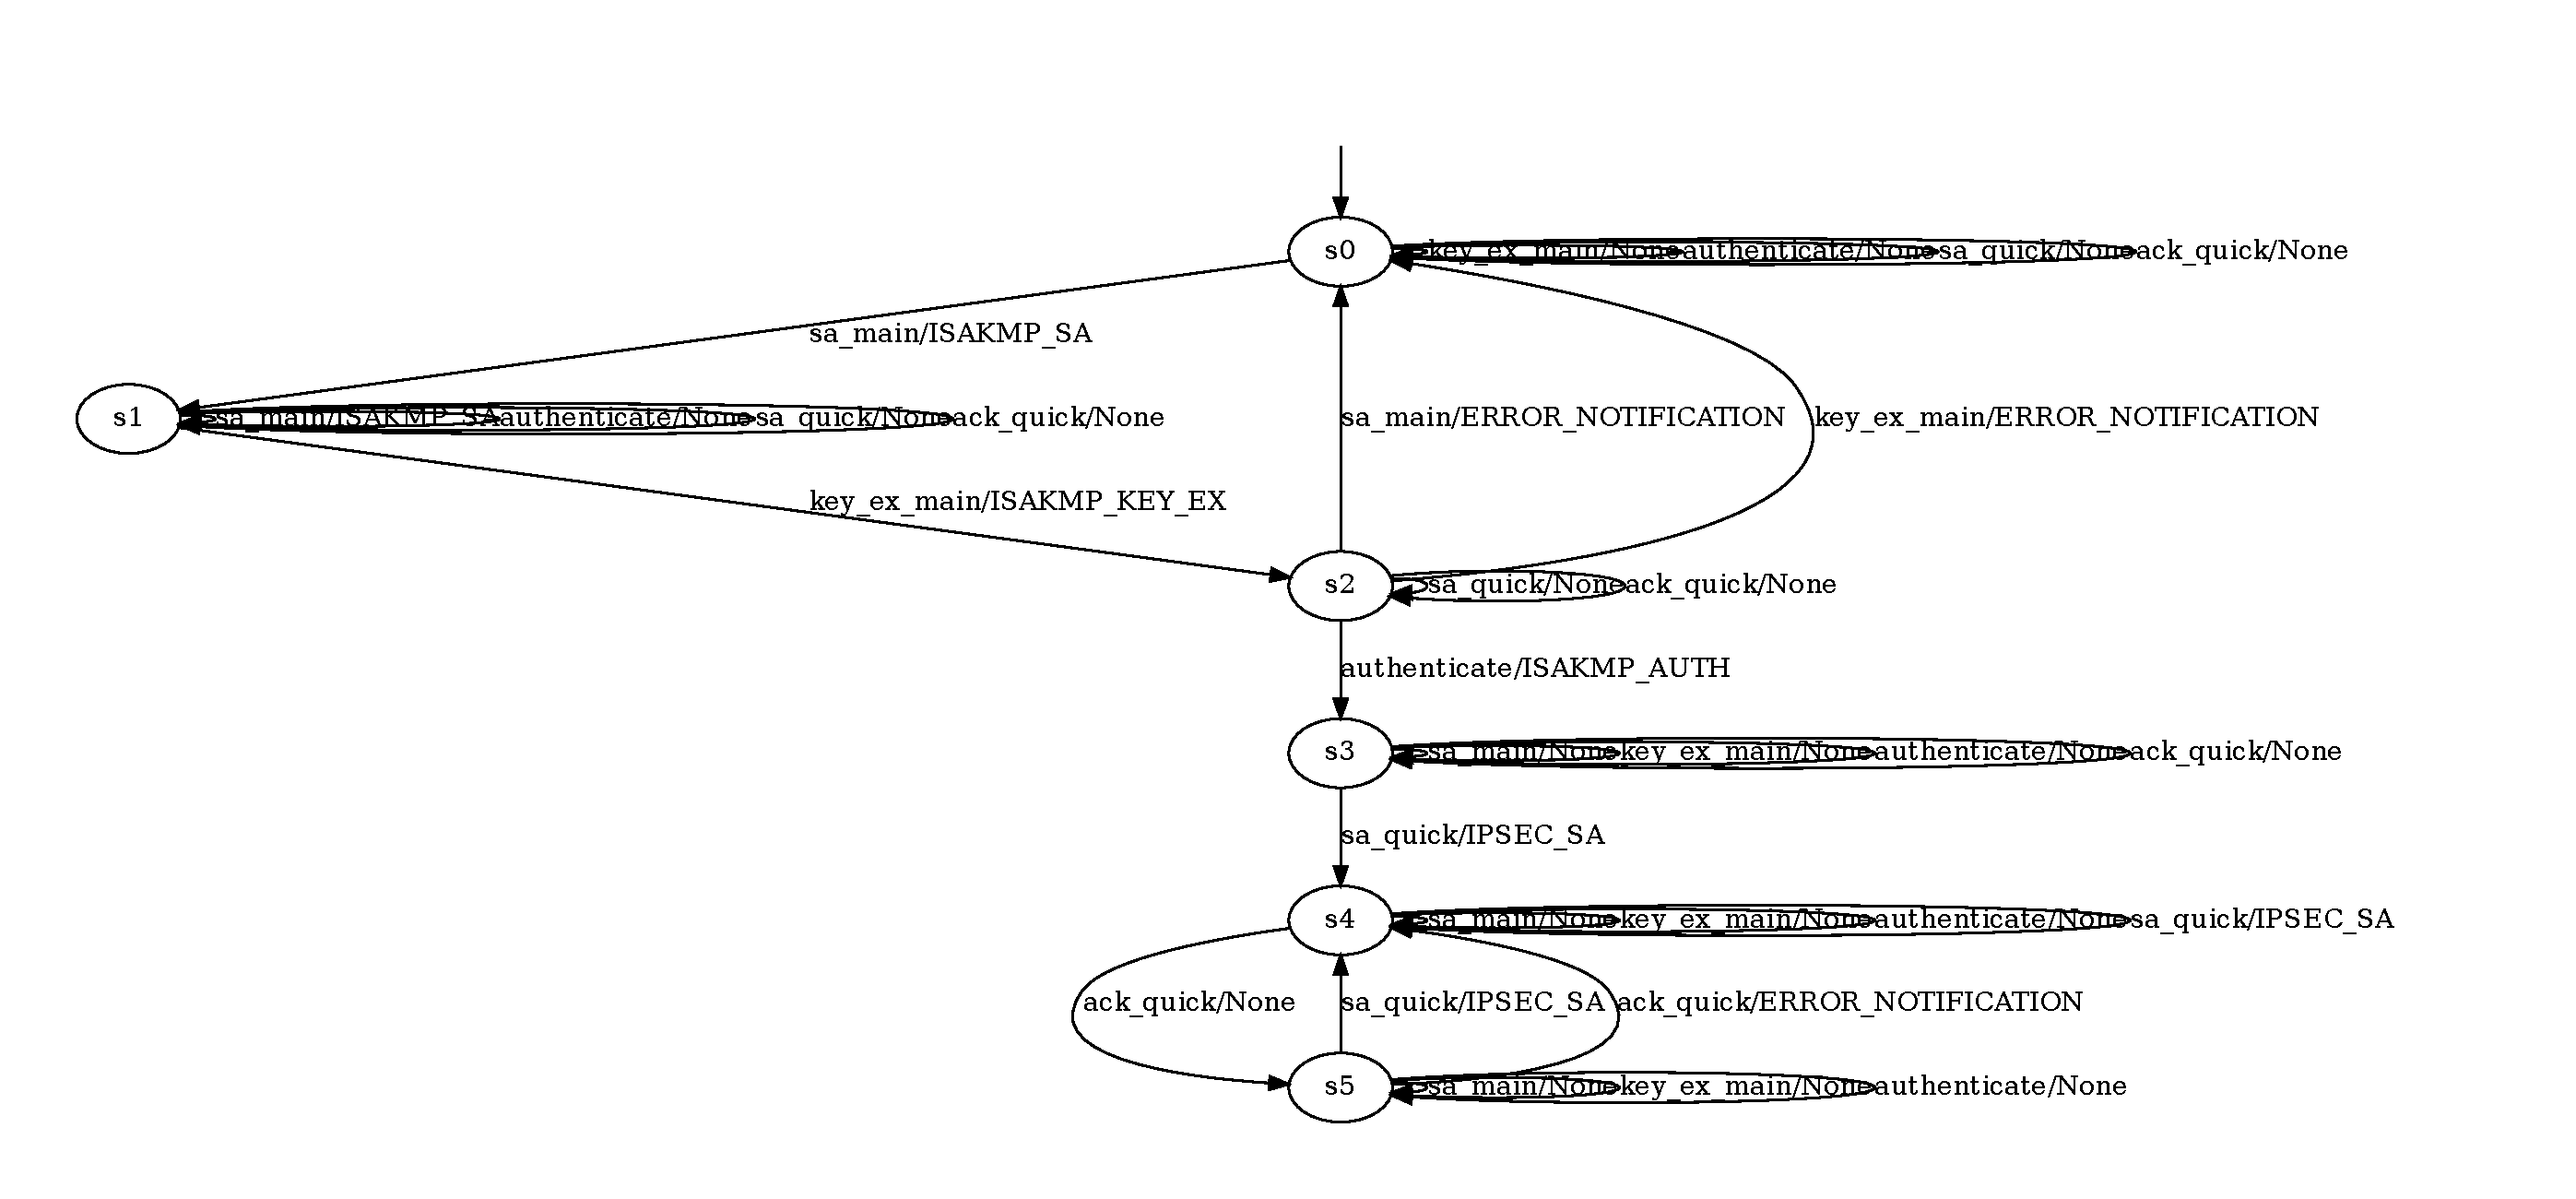
\includegraphics[width=\linewidth]{images/models/Reference}
	\caption{Clean model learned using retransmission filtering}
	\label{fig:reference}
\end{figure} 

\newpage


\subsubsection*{Fuzzing Reference Model}
\todo{stuff here}
% Error model
TODO: analyze error model
Figure \ref{fig:withfilterwitherrors} shows a model learned with retransmission-filtering enabled. Additionally, the input alphabet was expanded to include an additional erroneous version of each letter that maps to a malformed \ac{ike} message. This model served as the basis for our model-based fuzzing and was, thanks to the retransmission-filtering, 100\% deterministic. It took a total of 

The model looks largely identical to the previous model, apart from some additional self-transitions and one additional error transition from state \emph{s4} to \emph{s5}. Here, state \emph{s4} corresponds to the previous \emph{s6}. The error transition simply means that we need to create a valid \ac{ipsec} \ac{sa} before we can acknowledge it.

\begin{figure}
	\centering
	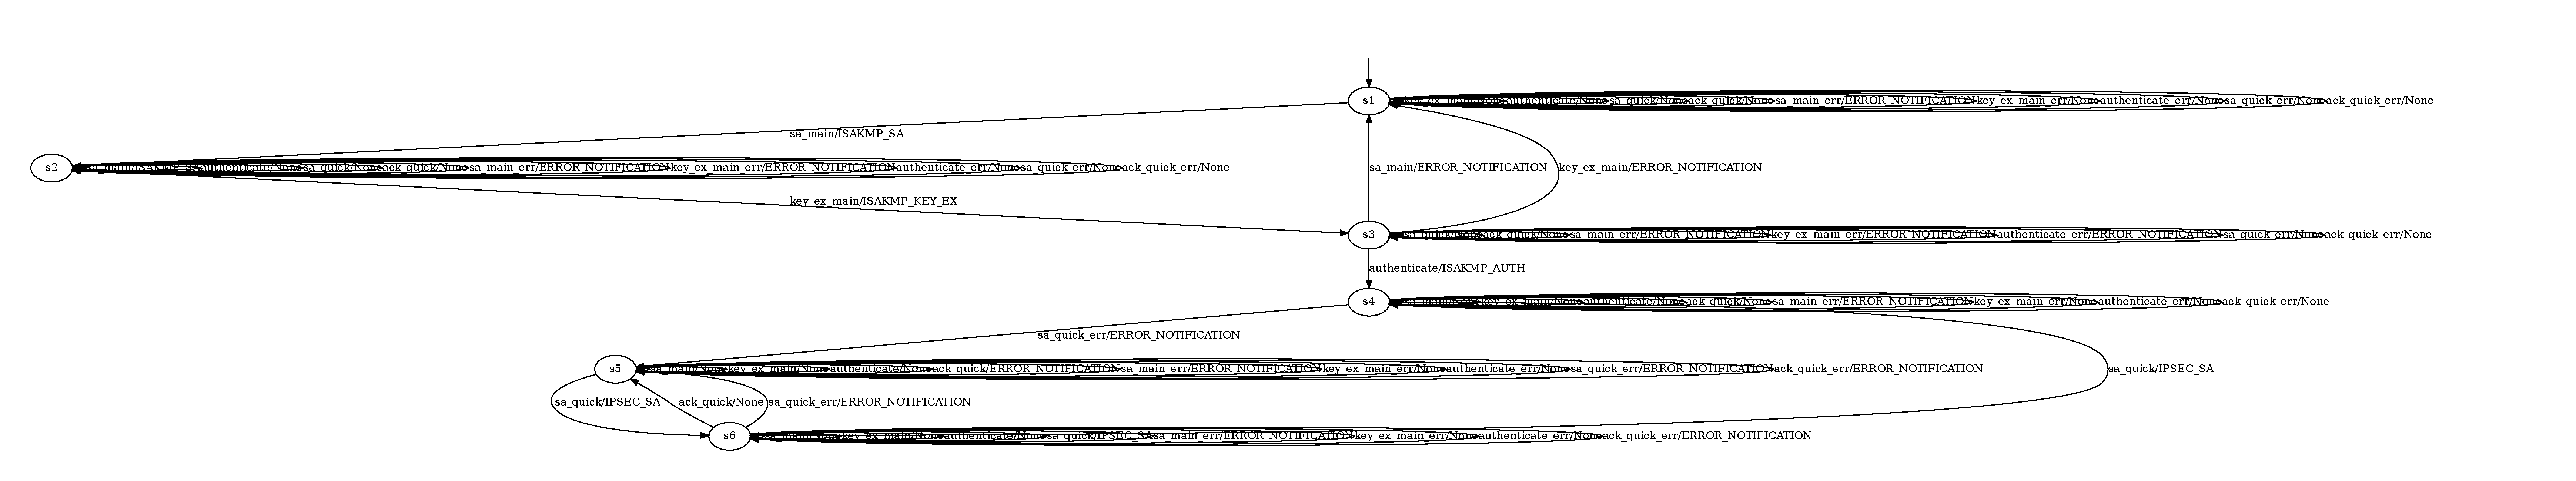
\includegraphics[width=\linewidth]{images/models/WithFilterWithErrors_kv}
	\caption{Model with malformed messages}
	\label{fig:withfilterwitherrors}
\end{figure}

\TODO{Do chart for each model}
\begin{table}[t]
	\centering
	\begin{tabular}{ |p{6.5cm}||p{1cm}|p{1cm}|  }
		\hline
		\multicolumn{3}{|c|}{\textbf{Learning Algorithm Performance (Averages) for Common Model A}} \\
		\hline
		\textbf{Metric} & $\mathbf{L^*}$ & $\mathbf{KV}$ \\
		\hline
		Learning Rounds							&	2				&	4 				\\
		Total Time (s)							&   3036			& 	2296   			\\
		Time Learning Algorithm	(s)				&	\textbf{1624}	& 	\textbf{879}	\\
		Time Equivalence Checks (s)				& 	1412			& 	1417			\\
		Learning Membership Queries 			&   \textbf{177}	& 	\textbf{79}		\\
		Learning Steps							& 	867	  			& 	753   			\\
		Equivalence Oracle Queries				& 	60  			&  	60				\\
		Equivalence Oracle Steps				& 	748  			&  	991				\\
		Membership Queries Saved by Caching		& 	14  			&  	27				\\
		\hline
	\end{tabular}
	\caption{Comparison $L^*$ and $KV$}
	\label{tab:commonmodel_a}
\end{table}

\subsection{Comparing $KV$ and $L^*$} \label{subsec:comp_kv_lstar}
% section copmaring KV and Lstar
Table \ref{tab:compkvlstar} shows average performance statistics over five learning runs each, with retransmission-filtering enabled. The same hardware and software configurations were used as described in Chapter \ref{sec:learnenv} with the learning program set up on a VirtualBox 6.1 \ac{vm} allotted 4GB of memory and one CPU core. We used all the basic packets for our input alphabet, so
\emph{sa\_main}, \emph{key\_ex\_main}, \emph{authenticate}, \emph{sa\_quick} and \emph{ack\_quick}. The model learned is the clean model seen in Figure \ref{fig:reference}. Table \ref{tab:compkvlstar} shows the metric on the left and the respective averages for the $L^*$ and $KV$ learning algorithms respectively on the right. Interesting results are highlighted in bold. From top to bottom, the metrics measured are as follows.
Learning rounds refers to the number of rounds the learning algorithms had to run for, or in other words, how many attempts they needed to correctly learn the \ac{sul}. Total time is the total time needed by the algorithm from start to the finished model. The total time can be split into time spent on the learning algorithm and time spent on equivalence queries. Learning membership queries refers to the number of membership queries sent to the SUL while learning steps to the steps in the learning algorithm itself. Analogously, equivalence oracle queries refers to the equivalence queries sent to the SUL and equivalence oracle steps to the steps needed by the equivalence oracle implementation. Finally, membership queries saved by caching details the performance boost gained by caching membership queries, with the value indicating the number of queries saved.

As the only difference between the two configurations tested was the choice of learning algorithm, intuitively we expect relevant fields to vary the most with equivalence oracle field to be largely unchanged. This intuition is confirmed by our experiments, wherein while the time spent on equivalence queries was very similar, the time spent on membership queries differed greatly. The $L^*$ algorithm required more than double the number of membership queries than its $KV$ counterpart. As membership queries are the main performance bottleneck in our setup, this change of course led to a significantly better runtime for $KV$, with total time spent on the learning algorithm being close to half that of the $L^*$ algorithm. This difference in time spent on the learning algorithm meant, that for this experiment, the $KV$ algorithm learned a model in roughly 75\% of the time needed by the $L^*$ algorithm. Looking only at the learning algorithm, $KV$ performed roughly twice as well as its counterpart.

Little variance was observed throughout previous learning attempts so this small sample size is believed to be representative. However, for even more accurate results the experiment should be carried out again for more runs. 

\todo{Redo with results from 20 runs. And detail standard deviation and such statistics.}

\begin{table}[t]
	\centering
	\begin{tabular}{ |p{6.5cm}||p{1cm}|p{1cm}|  }
		\hline
		\multicolumn{3}{|c|}{\textbf{Learning Algorithm Performance (Averages)}} \\
		\hline
		\textbf{Metric} & $\mathbf{L^*}$ & $\mathbf{KV}$ \\
		\hline
		Learning Rounds							&	2				&	4 				\\
		Total Time (s)							&   3036			& 	2296   			\\
		Time Learning Algorithm	(s)				&	\textbf{1624}	& 	\textbf{879}	\\
		Time Equivalence Checks (s)				& 	1412			& 	1417			\\
		Learning Membership Queries 			&   \textbf{177}	& 	\textbf{79}		\\
		Learning Steps							& 	867	  			& 	753   			\\
		Equivalence Oracle Queries				& 	60  			&  	60				\\
		Equivalence Oracle Steps				& 	748  			&  	991				\\
		Membership Queries Saved by Caching		& 	14  			&  	27				\\
		\hline
	\end{tabular}
	\caption{Comparison $L^*$ and $KV$}
	\label{tab:compkvlstar}
\end{table}

\subsection{Library Error} \label{subsec:liberror}
% section with discovered bug
Another notable finding from the model learning phase, was the discovery of a bug in a used Python Diffie-Hellman key exchange library. The bug was only found thanks to the exhaustive number of packets sent with our mapper class and due to the non-determinism checks implemented in \textsc{AALpy}. Despite our best efforts in removing the non-deterministic behavior from our learning process, we would still get occasional non-determinism errors at random points while learning. This problem persisted over several weeks due to the fact that the errors occurred randomly and only sporadically during some learning attempts. Initially we believed this to be also caused by retransmissions, but since the problems persisted even after introducing retransmission-filtering, that possibility was ruled out. The other option was of course problems in our implementation of the \ac{ipsec} protocol. Therefore, a lot of time was invested into painstakingly comparing logs and packet captures between our implementation and the \ac{sul} to ensure that everything lined up, since \textsc{AALpy} was still reporting non-determinism errors. Finally we discovered a discrepancy between the two and through it, that the problems were not in fact caused by our implementation, but by a used Python library. It turns out there was a very niche bug in a used Diffie-Hellman Python library where, if the most significant byte was a zero, it would be omitted from the response, causing the local result to be one byte shorter than the value calculated by the \ac{sul}. As this would only occur in the rare case where the MSB of the DH exchange was zero, this explains the random and difficult to reproduce nature of the bug. This behavior was undocumented and happened in a function call that allowed specifying the length of the returned key. As the library is not a very widespread one, the impact of this bug is presumably not very high. Regardless, it could compromise the security of affected systems and therefore the maintainer of the library has been notified of the problem. Due to the elusive nature of this bug, it would very likely not have been noticed without the exhaustive communication done by the model learning process and without seeing the slight differences in the resulting models that did not crash during the learning process.

\section{Fuzzing Results} \label{subsec:fuzzresults}
\todo[inline]{Fuzzing results}
\todo[inline]{Compare mutation based fuzzing and filtering results / runtimes}